\documentclass[11pt]{article}
\usepackage[a4paper,margin=22mm]{geometry}
\usepackage{amsmath,amssymb,booktabs,longtable,array,enumitem,graphicx,xcolor}
\usepackage[hidelinks]{hyperref}
\usepackage{tikz}
\usetikzlibrary{arrows.meta,positioning,calc,shapes.geometric}
\setlength{\parindent}{0pt}
\setlength{\parskip}{6pt}
\setlist[itemize]{nosep}
\setlist[enumerate]{itemsep=3pt}
\newcommand{\sol}{\paragraph{Solution.}}
\newcommand{\SA}{\mathrm{SA}}
\newcommand{\up}{\mathord{\Uparrow}}
\newcommand{\dn}{\mathord{\Downarrow}}
\newcommand{\any}{\mathord{\Updownarrow}}
\hypersetup{pdftitle={VLSI Testing: rebuilt examination and independent solutions},pdfauthor={}}
\begin{document}
\title{VLSI Testing: 2009 Midterm}\author{}\date{}\maketitle\begin{quote}\small
Reconstructed questions and independently derived solutions. Personal names, identifiers,
handwritten answers and administrative headers are omitted. Figures are redrawn as
logical diagrams or explicit netlists. A source-reading note identifies a meaningful
ambiguity instead of silently changing the question. Finite Boolean checks
are supplied in the examination collection's Python verification script.
\end{quote}

\section{SCOAP for two combinational circuits}
\textbf{Question.} Compute controllability and observability for
(a) the four-NAND XOR realization and (b) the AND--OR mux realization.
Input names below replace unlabeled input wires.

Use $CC_0=CC_1=1$ at a primary input and $CO=0$ at a primary output;
each gate adds one. For an AND gate,
$CC_0=1+\min CC_0(i)$ and $CC_1=1+\sum CC_1(i)$.
For an OR gate, interchange the roles of 0 and 1.
NAND/NOR swap the two output controllabilities; an inverter swaps its input
values and adds one. To observe one gate input, set the other inputs to their
noncontrolling values, add their controllability costs, add $CO$ of the output
and add one. At a fanout stem take the minimum branch $CO$.
For XOR/XNOR, minimize the sum of input costs subject to the desired parity.
These are structural SCOAP estimates; reconvergent inputs are treated independently.
\begin{center}\begin{tabular}{ll}\toprule Signal & Defining expression\\\midrule
$n$ & $\overline{AB}$\\
$u$ & $\overline{An}$\\
$v$ & $\overline{Bn}$\\
$Z$ & $\overline{uv}$\\
\bottomrule\end{tabular}\end{center}
\begin{center}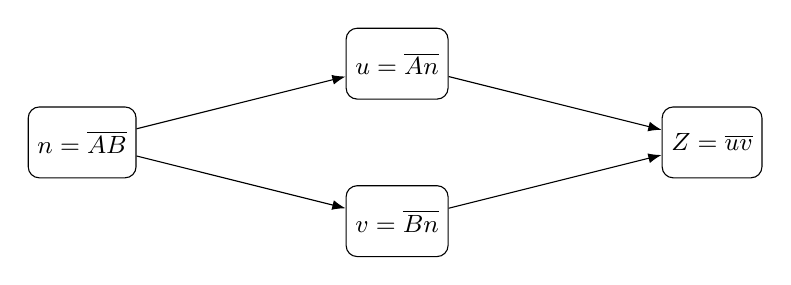
\begin{tikzpicture}[>=Latex,box/.style={draw,rounded corners,align=center,minimum height=9mm,font=\small},scale=1,transform shape]
\node[box] (n) at (0,0) {$n=\overline{AB}$};
\node[box] (u) at (4,1) {$u=\overline{An}$};
\node[box] (vv) at (4,-1) {$v=\overline{Bn}$};
\node[box] (z) at (8,0) {$Z=\overline{uv}$};
\draw[->] (n) -- (u);
\draw[->] (n) -- (vv);
\draw[->] (u) -- (z);
\draw[->] (vv) -- (z);
\end{tikzpicture}\end{center}
\begin{center}\begin{tabular}{lrrr}\toprule
Signal & $CC_0$ & $CC_1$ & $CO$\\\midrule
$A$ & 1 & 1 & 6\\
$B$ & 1 & 1 & 6\\
$n$ & 3 & 2 & 5\\
$u$ & 4 & 2 & 3\\
$v$ & 4 & 2 & 3\\
$Z$ & 5 & 5 & 0\\
\bottomrule\end{tabular}\end{center}

The $A,B$ stems each have $CO=6$; their branches into the first NAND
have $CO=7$. Branches into the second level have $CO=6$.
\begin{center}\begin{tabular}{ll}\toprule Signal & Defining expression\\\midrule
$n$ & $\bar S$\\
$u$ & $AS$\\
$v$ & $Bn$\\
$Z$ & $u+v$\\
\bottomrule\end{tabular}\end{center}
\begin{center}\begin{tabular}{lrrr}\toprule
Signal & $CC_0$ & $CC_1$ & $CO$\\\midrule
$A$ & 1 & 1 & 5\\
$S$ & 1 & 1 & 5\\
$B$ & 1 & 1 & 6\\
$n$ & 2 & 2 & 5\\
$u$ & 2 & 3 & 3\\
$v$ & 2 & 4 & 3\\
$Z$ & 5 & 4 & 0\\
\bottomrule\end{tabular}\end{center}

For (b), $CO(S\to u)=5$ and $CO(S\to n)=6$; take $CO(S)=5$.
The costs in (a) are structural estimates despite the function reducing to XOR.

\section{ATPG and pseudo-exhaustive testing}
\textbf{Question.} For the following circuit:
(a) find a D-algorithm test for $x/0$;
(b) find a single-path test for $y/0$;
(c) determine a pseudo-exhaustive test count.
The source also has a handwritten correction of (b) to $y/1$.
\begin{center}\begin{tabular}{ll}\toprule Signal & Defining expression\\\midrule
$p$ & $ABC$\\
$y$ & $EF$\\
$q$ & $\overline{Dy}$\\
$r$ & $HI$\\
$x$ & $r\text{ branch to the OR gate}$\\
$S$ & $pq(G+x)$\\
$T$ & $rJ$\\
\bottomrule\end{tabular}\end{center}
\begin{center}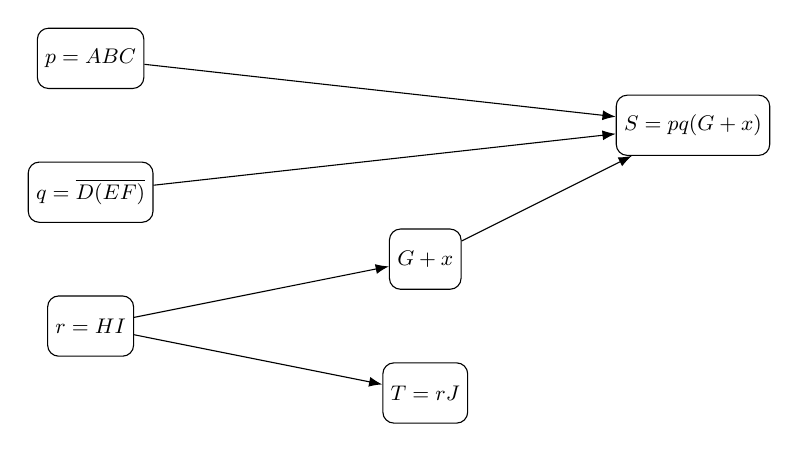
\begin{tikzpicture}[>=Latex,box/.style={draw,rounded corners,align=center,minimum height=9mm,font=\small},scale=0.85,transform shape]
\node[box] (p) at (0,2) {$p=ABC$};
\node[box] (q) at (0,0) {$q=\overline{D(EF)}$};
\node[box] (r) at (0,-2) {$r=HI$};
\node[box] (oo) at (5,-1) {$G+x$};
\node[box] (s) at (9,1) {$S=pq(G+x)$};
\node[box] (t) at (5,-3) {$T=rJ$};
\draw[->] (p) -- (s);
\draw[->] (q) -- (s);
\draw[->] (r) -- (oo);
\draw[->] (oo) -- (s);
\draw[->] (r) -- (t);
\end{tikzpicture}\end{center}

\sol For $x/0$, set $H=I=1$ so $x=D$, $G=0$ to propagate through OR,
$A=B=C=1$ and $D=0$ to make $p=q=1$.
For example $(A,B,C,D,E,F,G,H,I,J)=1110000110$ gives $S=1/0$.
For the printed $y/0$, set $E=F=D=1$, $A=B=C=1$, $G=1$.
Test $1111111000$ makes the NAND and $S$ change from 0 to 1.
For the handwritten $y/1$, test $1111001000$ gives $S=1/0$.
Thus both readings are solved rather than silently replacing the printed fault.

The $S$ cone depends on nine inputs $A,\ldots,I$. Exhaust their $2^9=512$
combinations. Choose $J=A$; then $(H,I,J)$ also covers all eight combinations
of the $T$ cone. This is a sufficient conventional pseudo-exhaustive
construction, not a proof of a minimum compressed test count.

\section{Equivalence and dominance}
\textbf{Question.} For $d=\overline{ab}$ and $e=\overline{d+c}$, classify
$a/0$, $b/1$, $d/1$ and $e/0$ by equivalence and dominance.
\begin{center}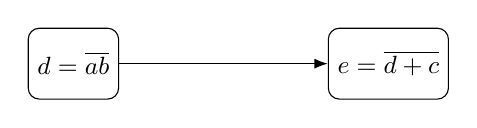
\begin{tikzpicture}[>=Latex,box/.style={draw,rounded corners,align=center,minimum height=9mm,font=\small},scale=1,transform shape]
\node[box] (d) at (0,0) {$d=\overline{ab}$};
\node[box] (e) at (4,0) {$e=\overline{d+c}$};
\draw[->] (d) -- (e);
\end{tikzpicture}\end{center}

\sol Since $e=ab\bar c$, the detection sets, in $(a,b,c)$ order, are
\[
T(a/0)=T(d/1)=T(e/0)=\{110\},\qquad T(b/1)=\{100\}.
\]
Thus the first three faults are equivalent. The fourth is neither equivalent to
nor in a strict dominance relationship with them: the two nonempty detection
sets are disjoint. Stating the sets also avoids opposite conventions for dominance.

\section{BDD and tests for a mux network}
\textbf{Question.} Two identical muxes with data $A_0,A_1$ and select $S_A$
feed a final mux selected by $S$.
(a) Build a BDD using one 0 leaf and one 1 leaf.
(b) Find all tests for the primary-output stuck-at faults.
The source crosses out \emph{outputs} and writes \emph{inputs}; solve both.
\begin{center}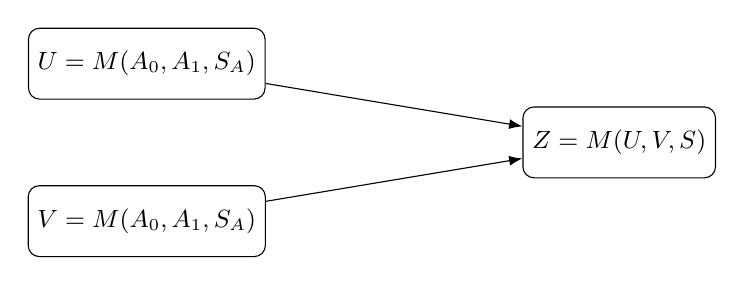
\begin{tikzpicture}[>=Latex,box/.style={draw,rounded corners,align=center,minimum height=9mm,font=\small},scale=1,transform shape]
\node[box] (u) at (0,1) {$U=M(A_0,A_1,S_A)$};
\node[box] (vv) at (0,-1) {$V=M(A_0,A_1,S_A)$};
\node[box] (z) at (6,0) {$Z=M(U,V,S)$};
\draw[->] (u) -- (z);
\draw[->] (vv) -- (z);
\end{tikzpicture}\end{center}

\sol The final data inputs are equal:
$Z=\bar S_A A_0+S_A A_1$, independent of $S$.
A reduced ordered BDD with order $S_A,A_0,A_1$ is:
\begin{center}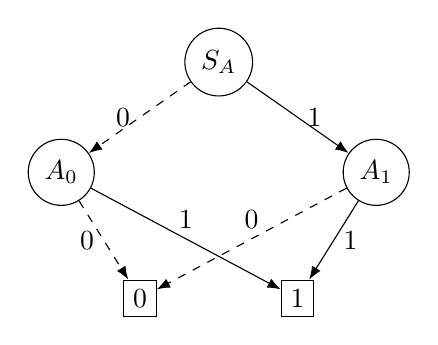
\begin{tikzpicture}[>=Latex]
\node[draw,circle](s) at(0,0){$S_A$};
\node[draw,circle](a)at(-2,-1.4){$A_0$};
\node[draw,circle](b)at(2,-1.4){$A_1$};
\node[draw,rectangle](z)at(-1,-3){0};
\node[draw,rectangle](o)at(1,-3){1};
\draw[->,dashed](s)--node[left]{0}(a);
\draw[->](s)--node[right]{1}(b);
\draw[->,dashed](a)--node[left]{0}(z);
\draw[->](a)--node[above]{1}(o);
\draw[->,dashed](b)--node[above]{0}(z);
\draw[->](b)--node[right]{1}(o);
\end{tikzpicture}\end{center}
Output-fault tests are $T(Z/0)=\{Z=1\}$ and $T(Z/1)=\{Z=0\}$.
For input stem faults, with unmentioned variables arbitrary:
\begin{center}\begin{tabular}{ll}\toprule Fault & All detecting assignments\\\midrule
$A_0/0$ & $S_A=0,A_0=1$\\
$A_0/1$ & $S_A=0,A_0=0$\\
$A_1/0$ & $S_A=1,A_1=1$\\
$A_1/1$ & $S_A=1,A_1=0$\\
$S_A/0$ & $S_A=1,A_0\ne A_1$\\
$S_A/1$ & $S_A=0,A_0\ne A_1$\\
$S/0,\ S/1$ & no tests (redundant select)\\\bottomrule
\end{tabular}\end{center}

\section{A hidden gate-level mux fault}
\textbf{Question.} A mux is realized by $C=A\,Sel$, $n=\overline{Sel}$,
$D=B n$, $Z=C+D$. Find a functional-block pin test set covering all
pin SA0/SA1 faults but missing $n/1$ at the input of AND gate $D$.
\begin{center}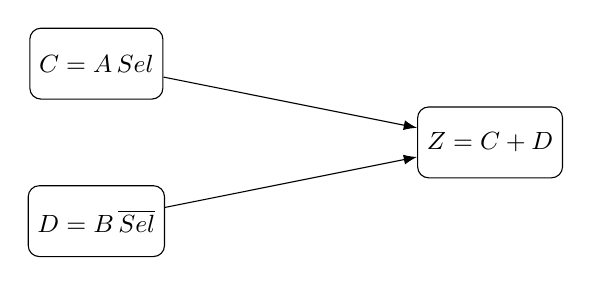
\begin{tikzpicture}[>=Latex,box/.style={draw,rounded corners,align=center,minimum height=9mm,font=\small},scale=1,transform shape]
\node[box] (c) at (0,1) {$C=A\,Sel$};
\node[box] (d) at (0,-1) {$D=B\,\overline{Sel}$};
\node[box] (z) at (5,0) {$Z=C+D$};
\draw[->] (c) -- (z);
\draw[->] (d) -- (z);
\end{tikzpicture}\end{center}

\sol In $(A,B,Sel)$ order use $\{000,001,010,101\}$, with outputs $0,0,1,1$.
$A/0$ is detected by 101, $A/1$ by 001, $B/0$ by 010, $B/1$ by 000,
$Sel/0$ by 101 and $Sel/1$ by 010. Both output faults are covered.
However $n/1$ is detected only by $Sel=1,B=1,A=0$, namely 011, which is absent.
Functional pin coverage does not imply internal structural coverage.

\section{XOR deductive simulation and a half-adder}
\textbf{Question.} Give a general XOR deductive rule and simulate
$S=A\oplus B$, $C=AB$ under inputs 01 and 10.
\sol A fault in an odd number of XOR-input fault lists changes parity.
Hence $L(S)=L(A)\mathbin{\triangle}L(B)$, followed by insertion of the
locally excited output stuck-at fault. For $m$ inputs take the symmetric
difference of all $m$ lists. A fault common to two lists cancels.
With signal-stem SA0/SA1 faults:
\begin{center}\begin{tabular}{lll}\toprule Input & $L(S)$ & $L(C)$\\\midrule
01 & $\{A/1,B/0,S/0\}$ & $\{A/1,C/1\}$\\
10 & $\{A/0,B/1,S/0\}$ & $\{B/1,C/1\}$\\\bottomrule
\end{tabular}\end{center}
\begin{center}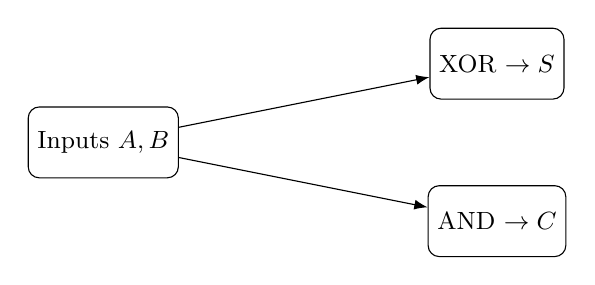
\begin{tikzpicture}[>=Latex,box/.style={draw,rounded corners,align=center,minimum height=9mm,font=\small},scale=1,transform shape]
\node[box] (a) at (0,0) {Inputs $A,B$};
\node[box] (s) at (5,1) {XOR $\to S$};
\node[box] (c) at (5,-1) {AND $\to C$};
\draw[->] (a) -- (s);
\draw[->] (a) -- (c);
\end{tikzpicture}\end{center}

\section{Short questions on manufacturing test}
\begin{enumerate}[label=(\alph*)]
\item \textbf{Verification and test.} Verification asks whether the design implements
the specification. Manufacturing test applies stimuli to fabricated hardware and
checks for physical defects represented by a fault model.
\item \textbf{Yield and defect level.} With yield $Y=0.5$, use the model
$DL=1-Y^{1-FC}$ for the defect fraction among shipped parts.
For $DL\le100\times10^{-6}$,
\[
 FC\ge1-\frac{\ln(0.9999)}{\ln(0.5)}
 =0.99985572\ldots,
\]
so at least $99.9856\%$ fault coverage is required \emph{under this model}.
Yield alone cannot determine defect level without a coverage/escape model.
\item \textbf{Test flow.} Select a defect/fault model; generate and simulate tests;
prepare tester programs and expected responses; apply tests at wafer/package/board
stages as appropriate; compare responses, diagnose failures and bin devices;
feed results back to design and manufacturing.
\item \textbf{Detection, location, diagnosis.} Detection distinguishes faulty from
fault-free behavior. Location narrows the physical or logical site. Diagnosis
infers likely fault mechanisms/sites from the response syndrome.
\item \textbf{Fault modeling.} A finite logical/electrical abstraction of defects makes
test generation and coverage measurable; model coverage need not equal defect coverage.
\item \textbf{Bathtub curve.} Early failures decrease as weak parts fail;
useful life has a low approximately constant hazard;
wear-out failures increase with aging.
\item \textbf{Fault coverage.} $FC=N_{\rm detected}/N_{\rm modeled}$, with the
denominator and any exclusion of untestable faults stated explicitly.
\item \textbf{Fault simulation.} Predict faulty responses, measure coverage, identify
undetected faults and grade/compact tests; optionally provide diagnostic signatures.
\end{enumerate}
\begin{center}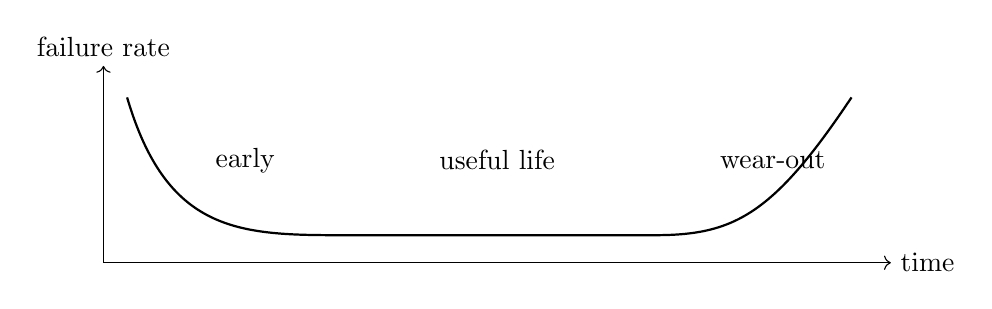
\begin{tikzpicture}[x=1cm,y=1cm]
\draw[->](0,0)--(10,0) node[right]{time};
\draw[->](0,0)--(0,2.5) node[above]{failure rate};
\draw[thick] (0.3,2.1) .. controls (.8,.4) and (1.7,.35) .. (3,.35)
 --(7,.35) .. controls(8,.35) and(8.5,.6) ..(9.5,2.1);
\node at(1.8,1.3){early};\node at(5,1.3){useful life};\node at(8.5,1.3){wear-out};
\end{tikzpicture}\end{center}

\section{Switch-level XNOR and stuck-open tests}
\textbf{Question.} Give a switch-level two-input XNOR. List all transistor
stuck-open faults requiring two-pattern tests, with the tests.
\sol Use two input inverters to supply $\bar A,\bar B$, and complementary
pull-down/pull-up networks:
\[
\mathrm{PDN}=(n_A\text{ series }n_{\bar B})
 \text{ parallel }(n_{\bar A}\text{ series }n_B),
\]
\[
\mathrm{PUN}=(p_A\text{ parallel }p_{\bar B})
 \text{ series }(p_{\bar A}\text{ parallel }p_B).
\]
Subscripts denote gate signals. NMOS conducts for 1; PMOS for 0.
This is an eight-transistor core plus four inverter transistors.
The PDN realizes XOR, so the output realizes XNOR.
\begin{center}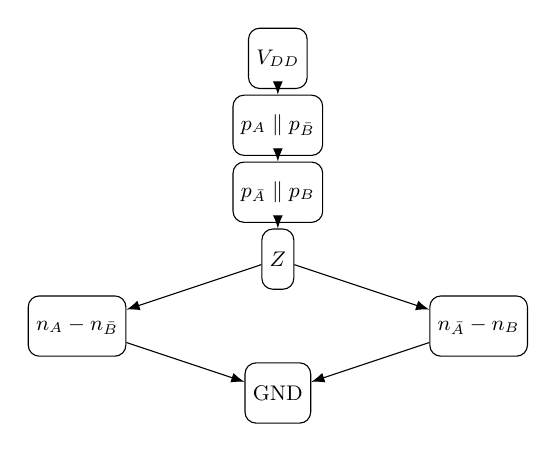
\begin{tikzpicture}[>=Latex,box/.style={draw,rounded corners,align=center,minimum height=9mm,font=\small},scale=0.85,transform shape]
\node[box] (vdd) at (0,2) {$V_{DD}$};
\node[box] (p1) at (0,1) {$p_A\parallel p_{\bar B}$};
\node[box] (p2) at (0,0) {$p_{\bar A}\parallel p_B$};
\node[box] (z) at (0,-1) {$Z$};
\node[box] (n1) at (-3,-2) {$n_A-n_{\bar B}$};
\node[box] (n2) at (3,-2) {$n_{\bar A}-n_B$};
\node[box] (gnd) at (0,-3) {GND};
\draw[->] (vdd) -- (p1);
\draw[->] (p1) -- (p2);
\draw[->] (p2) -- (z);
\draw[->] (z) -- (n1);
\draw[->] (z) -- (n2);
\draw[->] (n1) -- (gnd);
\draw[->] (n2) -- (gnd);
\end{tikzpicture}\end{center}

In the ideal charge-storage stuck-open model, initialize the output/internal
node and then require the missing path:
\begin{center}\begin{tabular}{ll}\toprule Open transistor(s) & $(A,B)_{\rm init}\to(A,B)_{\rm test}$\\\midrule
$p_A$ or $p_B$ & $01\to00$\\
$p_{\bar A}$ or $p_{\bar B}$ & $01\to11$\\
$n_A$ or $n_{\bar B}$ & $00\to10$\\
$n_{\bar A}$ or $n_B$ & $00\to01$\\
PMOS in $\bar A$ inverter & $11\to01$\\
NMOS in $\bar A$ inverter & $01\to11$\\
PMOS in $\bar B$ inverter & $11\to10$\\
NMOS in $\bar B$ inverter & $10\to11$\\\bottomrule
\end{tabular}\end{center}
For example $01\to00$ first discharges $Z$, then should charge it through
$p_A,p_B$. If either is open, $Z$ retains 0.
For inverter opens, the first vector initializes the complementary signal.
Charge sharing and leakage require electrical timing analysis beyond this model.

\end{document}
